\subsubsection{MOSFET tipo N e tipo P}

Os MOSFETs são dispositivos semicondutores cujo funcionamento é baseado no controle de um canal de condução por meio de um campo elétrico. Diferentemente dos BJTs, que dependem de uma corrente aplicada à base, os MOSFETs são controlados principalmente pela tensão entre os terminais gate e source ($V_{GS}$).

Sua estrutura possui quatro regiões principais: gate, source, drain e body (ou substrate). Em muitos componentes comerciais, o body é conectado internamente ao source, fazendo com que o dispositivo seja apresentado externamente com apenas três terminais.

O terminal gate é separado do semicondutor por uma camada isolante, tradicionalmente de dióxido de silício ($SiO_2$). Essa camada impede a passagem de corrente contínua significativa entre o gate e o restante do dispositivo, permitindo que a tensão aplicada ao gate produza um campo elétrico capaz de modificar a concentração de portadores de carga na região abaixo dele.

Existem dois tipos principais de MOSFETs:

\begin{figure}[H]
    \centering
    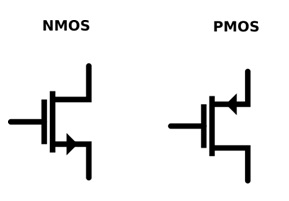
\includegraphics[width=0.6\linewidth]{images/NMOS-PMOS.jpg}
    \caption{Representação dos MOSFETs tipo N e tipo P}
    \label{nmos-pmos-transistors}
    {\footnotesize Fonte: \url{https://www.langirswitch.com}}
\end{figure}

\textbf{NMOS (N-channel MOSFET):} em um transistor NMOS de enriquecimento, uma tensão positiva suficientemente elevada entre gate e source ($V_{GS}$) cria um canal condutor do tipo N entre source e drain. Esse processo ocorre quando $V_{GS}$ ultrapassa a tensão de limiar ($V_{TH}$). Assim, o transistor passa a permitir a condução de corrente entre seus terminais.

\textbf{PMOS (P-channel MOSFET):} em um transistor PMOS de enriquecimento, o funcionamento é complementar. Uma tensão suficientemente negativa entre gate e source cria um canal condutor do tipo P. Portanto, o dispositivo entra em condução quando $V_{GS}$ é suficientemente menor que zero, em relação ao seu limiar de operação.

De maneira simplificada, considerando uma alimentação positiva ($V_{DD}$), o comportamento dos dois dispositivos pode ser descrito da seguinte maneira: o NMOS conduz quando o gate recebe um nível lógico alto e interrompe a condução quando recebe um nível lógico baixo, enquanto o PMOS conduz quando o gate recebe um nível lógico baixo e interrompe a condução quando recebe um nível lógico alto.
É importante destacar que o funcionamento depende da tensão entre gate e source, e não apenas da tensão absoluta do gate em relação ao GND.

\paragraph{Funcionamento físico do NMOS}

\begin{figure}[H]
    \centering
    \includegraphics[width=0.6\linewidth]{images/nmos.jpg}
    \caption{Diagrama do transistor NMOS de enriquecimento}
    \label{nmos-diagram}
    {\footnotesize Fonte: \url{https://dwma4bz18k1bd.cloudfront.net/tutorials/NMOS-Transistor-Structure.jpg}}
\end{figure}

Em um NMOS de enriquecimento, o substrato é geralmente do tipo P, enquanto as regiões de source e drain são dopadas com impurezas do tipo N.

Quando nenhuma tensão significativa é aplicada ao gate, não existe um canal condutor contínuo entre source e drain. As junções entre as regiões N e P impedem que exista um caminho de condução direta entre os dois terminais.

Quando uma tensão positiva é aplicada ao gate, o campo elétrico produzido atrai elétrons para a região superficial do substrato, abaixo da camada isolante. À medida que a tensão aumenta, a concentração de elétrons nessa região também aumenta.

Quando a tensão ultrapassa a tensão de limiar ($V_{TH}$), forma-se um canal de inversão do tipo N, conectando eletricamente as regiões de source e drain.

A partir desse momento, uma diferença de potencial entre source e drain permite a passagem de corrente elétrica através do canal.

\paragraph{Funcionamento físico do PMOS}

O PMOS apresenta uma estrutura complementar. Seu substrato é geralmente do tipo N, enquanto as regiões de source e drain são dopadas com impurezas do tipo P.

Quando uma tensão suficientemente negativa é aplicada ao gate em relação ao source, o campo elétrico favorece o acúmulo de lacunas na superfície do substrato.

Quando a tensão ultrapassa o limiar de operação do dispositivo, forma-se um canal de condução do tipo P entre source e drain.

Dessa maneira, o PMOS permite a condução de corrente quando seu gate apresenta uma tensão suficientemente inferior à tensão de source.

\paragraph{MOSFETs em circuitos digitais}

Em circuitos digitais, especialmente na tecnologia CMOS (\textit{Complementary Metal-Oxide-Semiconductor}), os transistores NMOS e PMOS são utilizados de forma complementar.

O NMOS é normalmente empregado para conectar a saída ao GND, enquanto o PMOS é utilizado para conectar a saída à alimentação positiva ($V_{DD}$).

Essa configuração permite construir circuitos lógicos nos quais a saída assume níveis de tensão próximos de GND ou $V_{DD}$, dependendo do estado das entradas.

Uma característica importante da tecnologia CMOS é que, em condições ideais de operação estática, não existe um caminho de condução direta entre a alimentação e o GND. Consequentemente, o consumo estático de potência é bastante reduzido, embora ainda exista consumo associado a correntes de fuga e outros efeitos não ideais.
